\subsubsection{The \emph{real} implemenation}

Eventually some code was developed  that handles a virtual disk. This code and
some details about the file format are described in this section.

\paragraph{The classes}

Figure \ref{fig:vfs_impl_classes} shows the overview over the classes
implemented for the disk handling and file management.


\begin{figure}[h!]
\centering
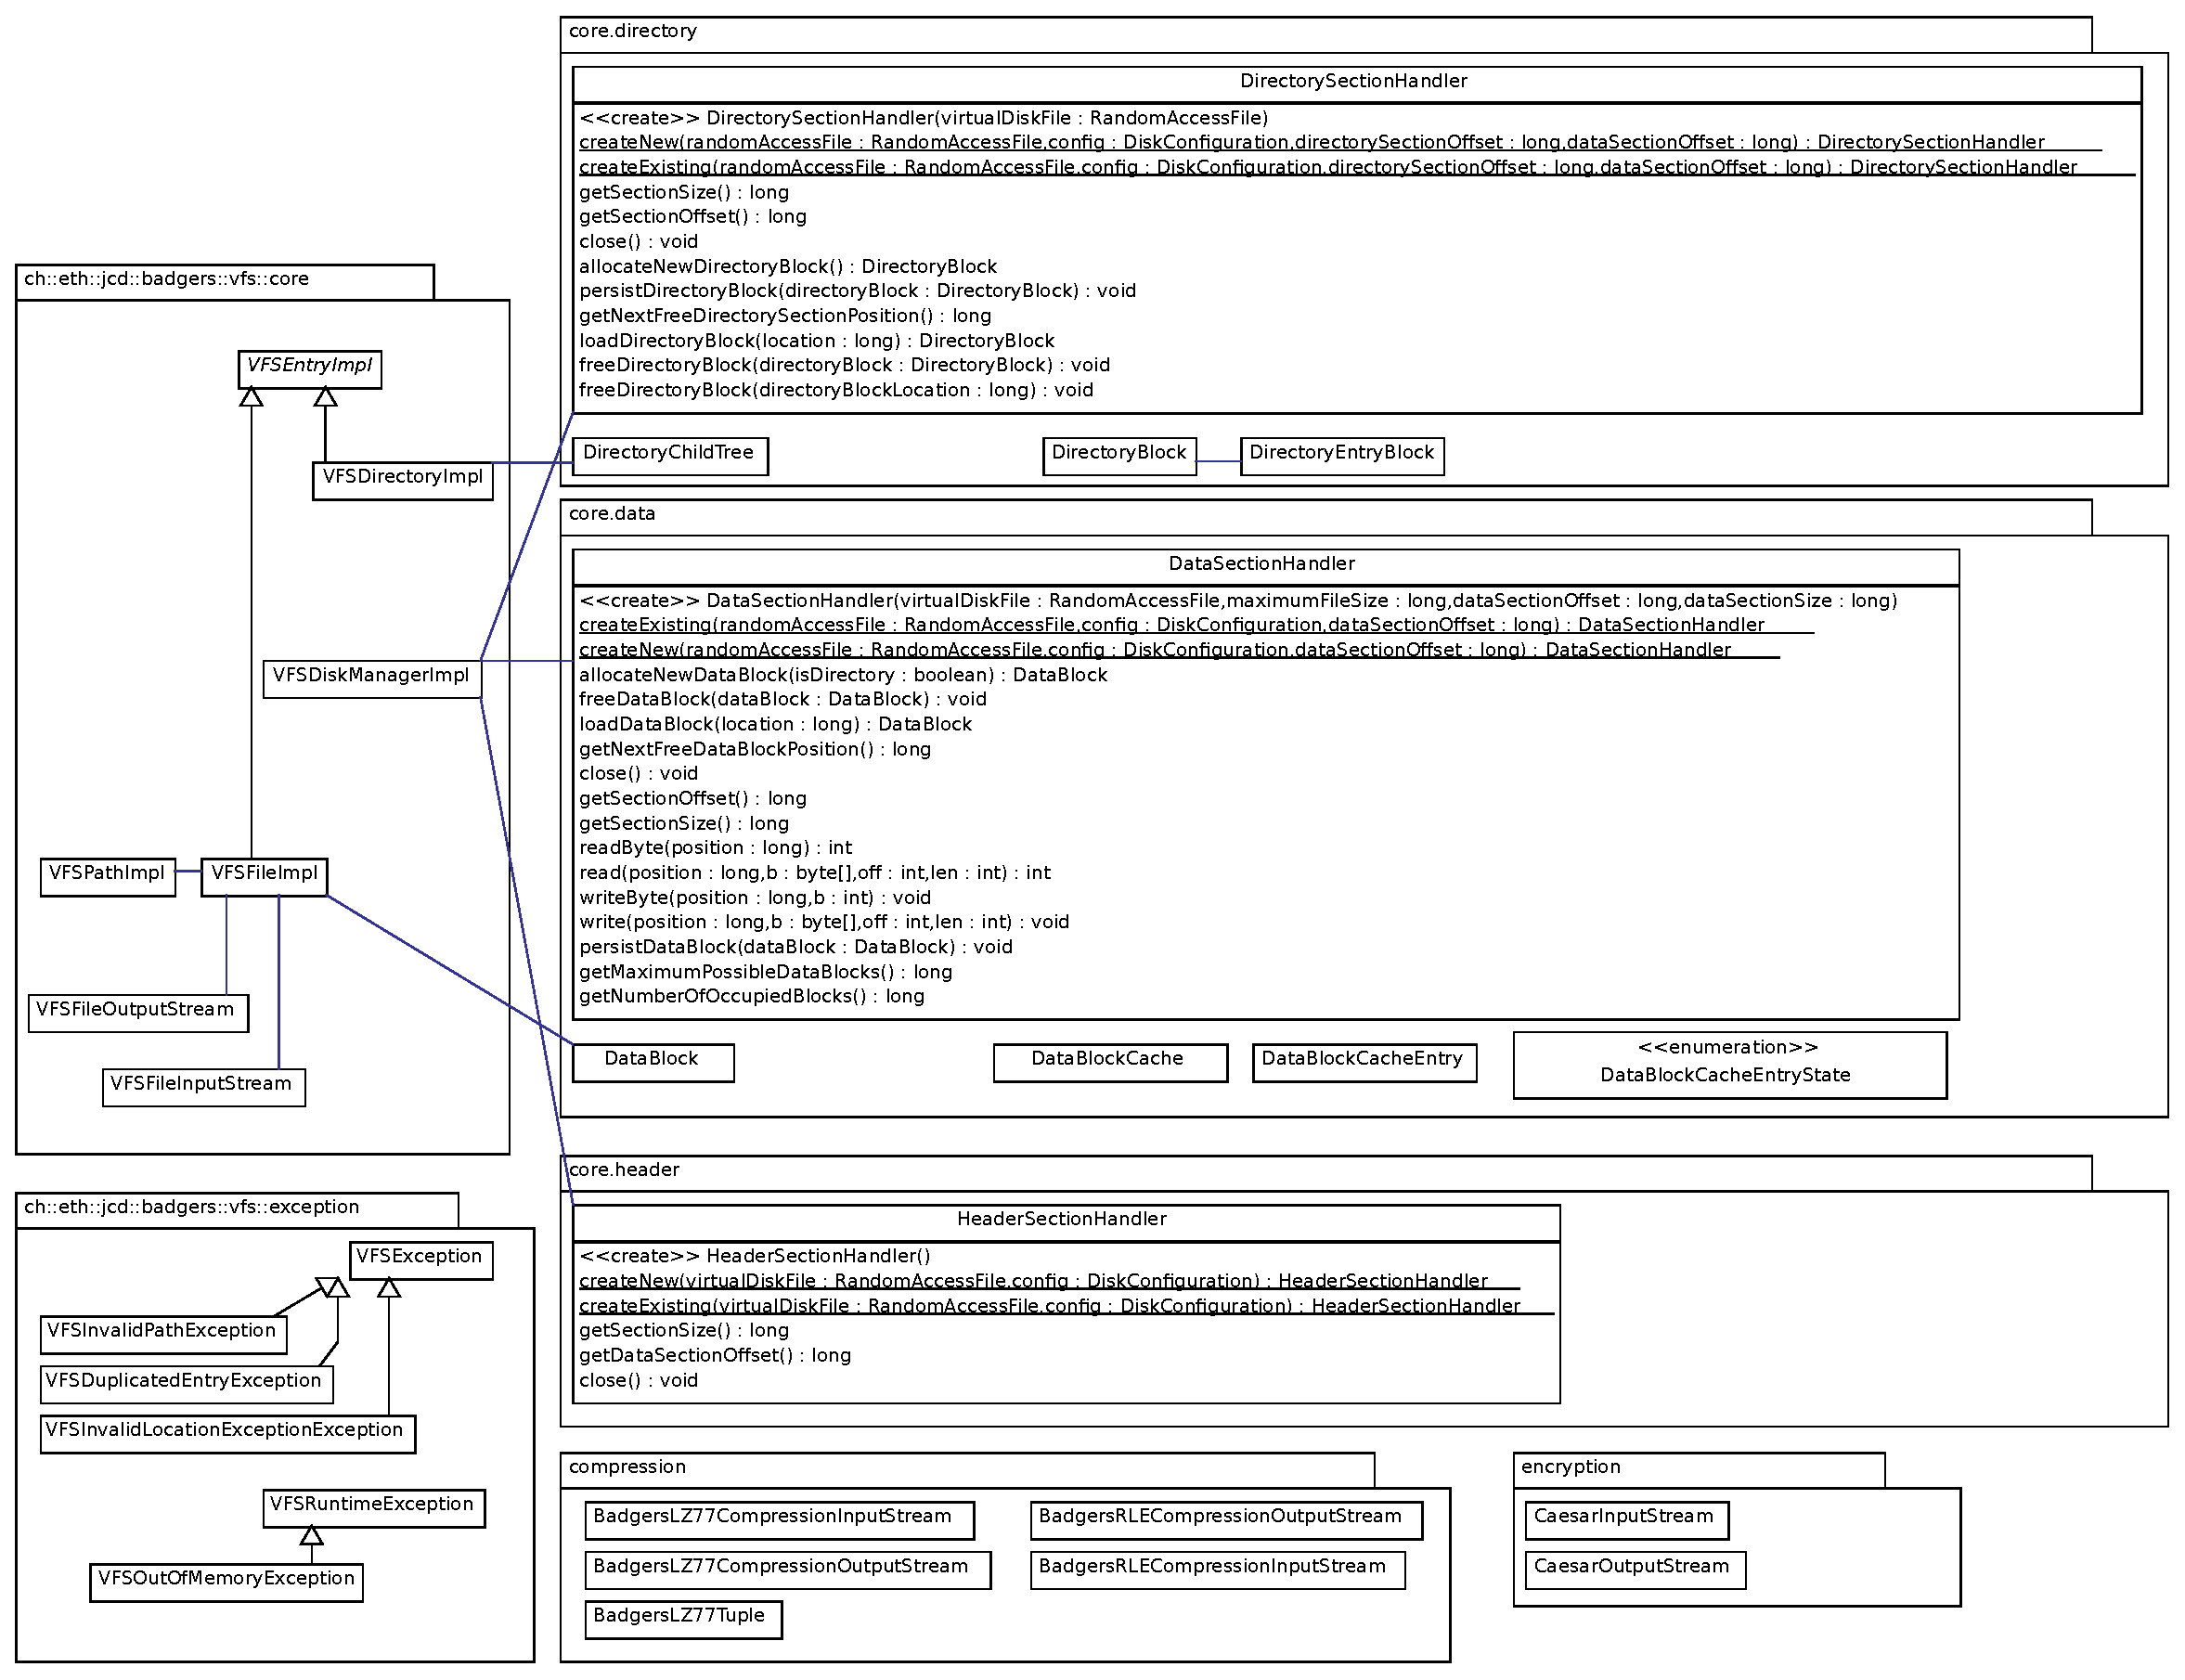
\includegraphics[width=1\textwidth]{figures/vfs_impl_classes.eps}
\caption{Implementation of the VFS core classes}
\label{fig:vfs_impl_classes}
\end{figure}

The classes were divided into several packages which are explained here in more
detail.

\subparagraph{core}
The \textit{core} package contains the implementation of the interfaces
mentioned in section \ref{sec:coreClasses}. Clients of the VFS core library operate on these
classes to manipulate the virtual file system.

\subparagraph{exception}
While manipulating the file system some exceptional behaviour might occur and
thus some exceptions will be thrown by the core classes. These exception are
propagated to the clients of the VFS core libraries.

\subparagraph{core.header}
As the virtual disk is divided into three sections (header, directory and data)
the classes that handle the management of the header section are put in the
package \textit{core.header}.
\subparagraph{core.data}
\textit{core.data} contains the classes that manipulate the data section on the
file system. This mainly means managing data blocks and actually writing/reading
the raw data bytes of files to the virtual disk.
\subparagraph{core.directory}
\textit{core.directory} contains the classes that manage the index of the file
system. That means that the whole directory structure is maintained in here.
This is done in a B-Tree that contains all references to directories and files
currently saved in the file system. More about the internals of directory
section can be found in section \ref{sec:file_format}

\subparagraph{encryption}
The encryption package shows some demo classes that implement a ceasar
cipher\footnote{http://en.wikipedia.org/wiki/Caesar\_cipher}. These classes are
mainly to show how encrpytion in VFS core can be implemented and configured. To
enable encryption in a new virtual disk one has to enable it in the
\textit{DiskConfiguration} that is passed to the \textit{VFSDiskManagerImpl} at
creation. Upon selecting the encryption algorithm the encryption stream will be
wrapped around the \textit{VFSFileInput- and VFSFileOutputStream}s.

\subparagraph{compression}

To reduce the data volume within the virtual disk, compression on each file can
be enabled. As mentioned earlier, compression is implemented as Input- and
OutputStreams and thus is wrapped around the \textit{VFSFileInput- and
VFSFileOutputStream}s. Currently available compression algorithms are run length
encoding \cite{rle} and LZ77 \cite{lz77}.

\begin{itemize}
  \item {\textit{Run Length Encoding}} The available 8bit run length
  encoding(rle) algorithm is a very simple form of data compression where
  multiple occurrence of the same byte were stored as a single byte value and
  the corresponding count. It is useful for simple graphic images like line
  drawings and icons.
  \item {\textit{LZ77}} Abraham Lempel and Jacob Ziv introduced the LZ77 lossless
  compression algorithm in 1977. Newer compression methods such as GZIP or DEFLATE often use LZ77-based
  algorithms. The compression is achieved by replacing the data with a reference
  to an earlier existing copy in the data input stream. For that a window of
  a certain size is held in memory where existing copies of the current data are
  searched.
\end{itemize}




\paragraph{The File Format}\label{sec:file_format}
This section describes the binary file format used by the file system inside a
virtual disk. The file is separated into three major parts. The header, index
and the data section. Each of them is described below.

\begin{figure}[h!]
\centering
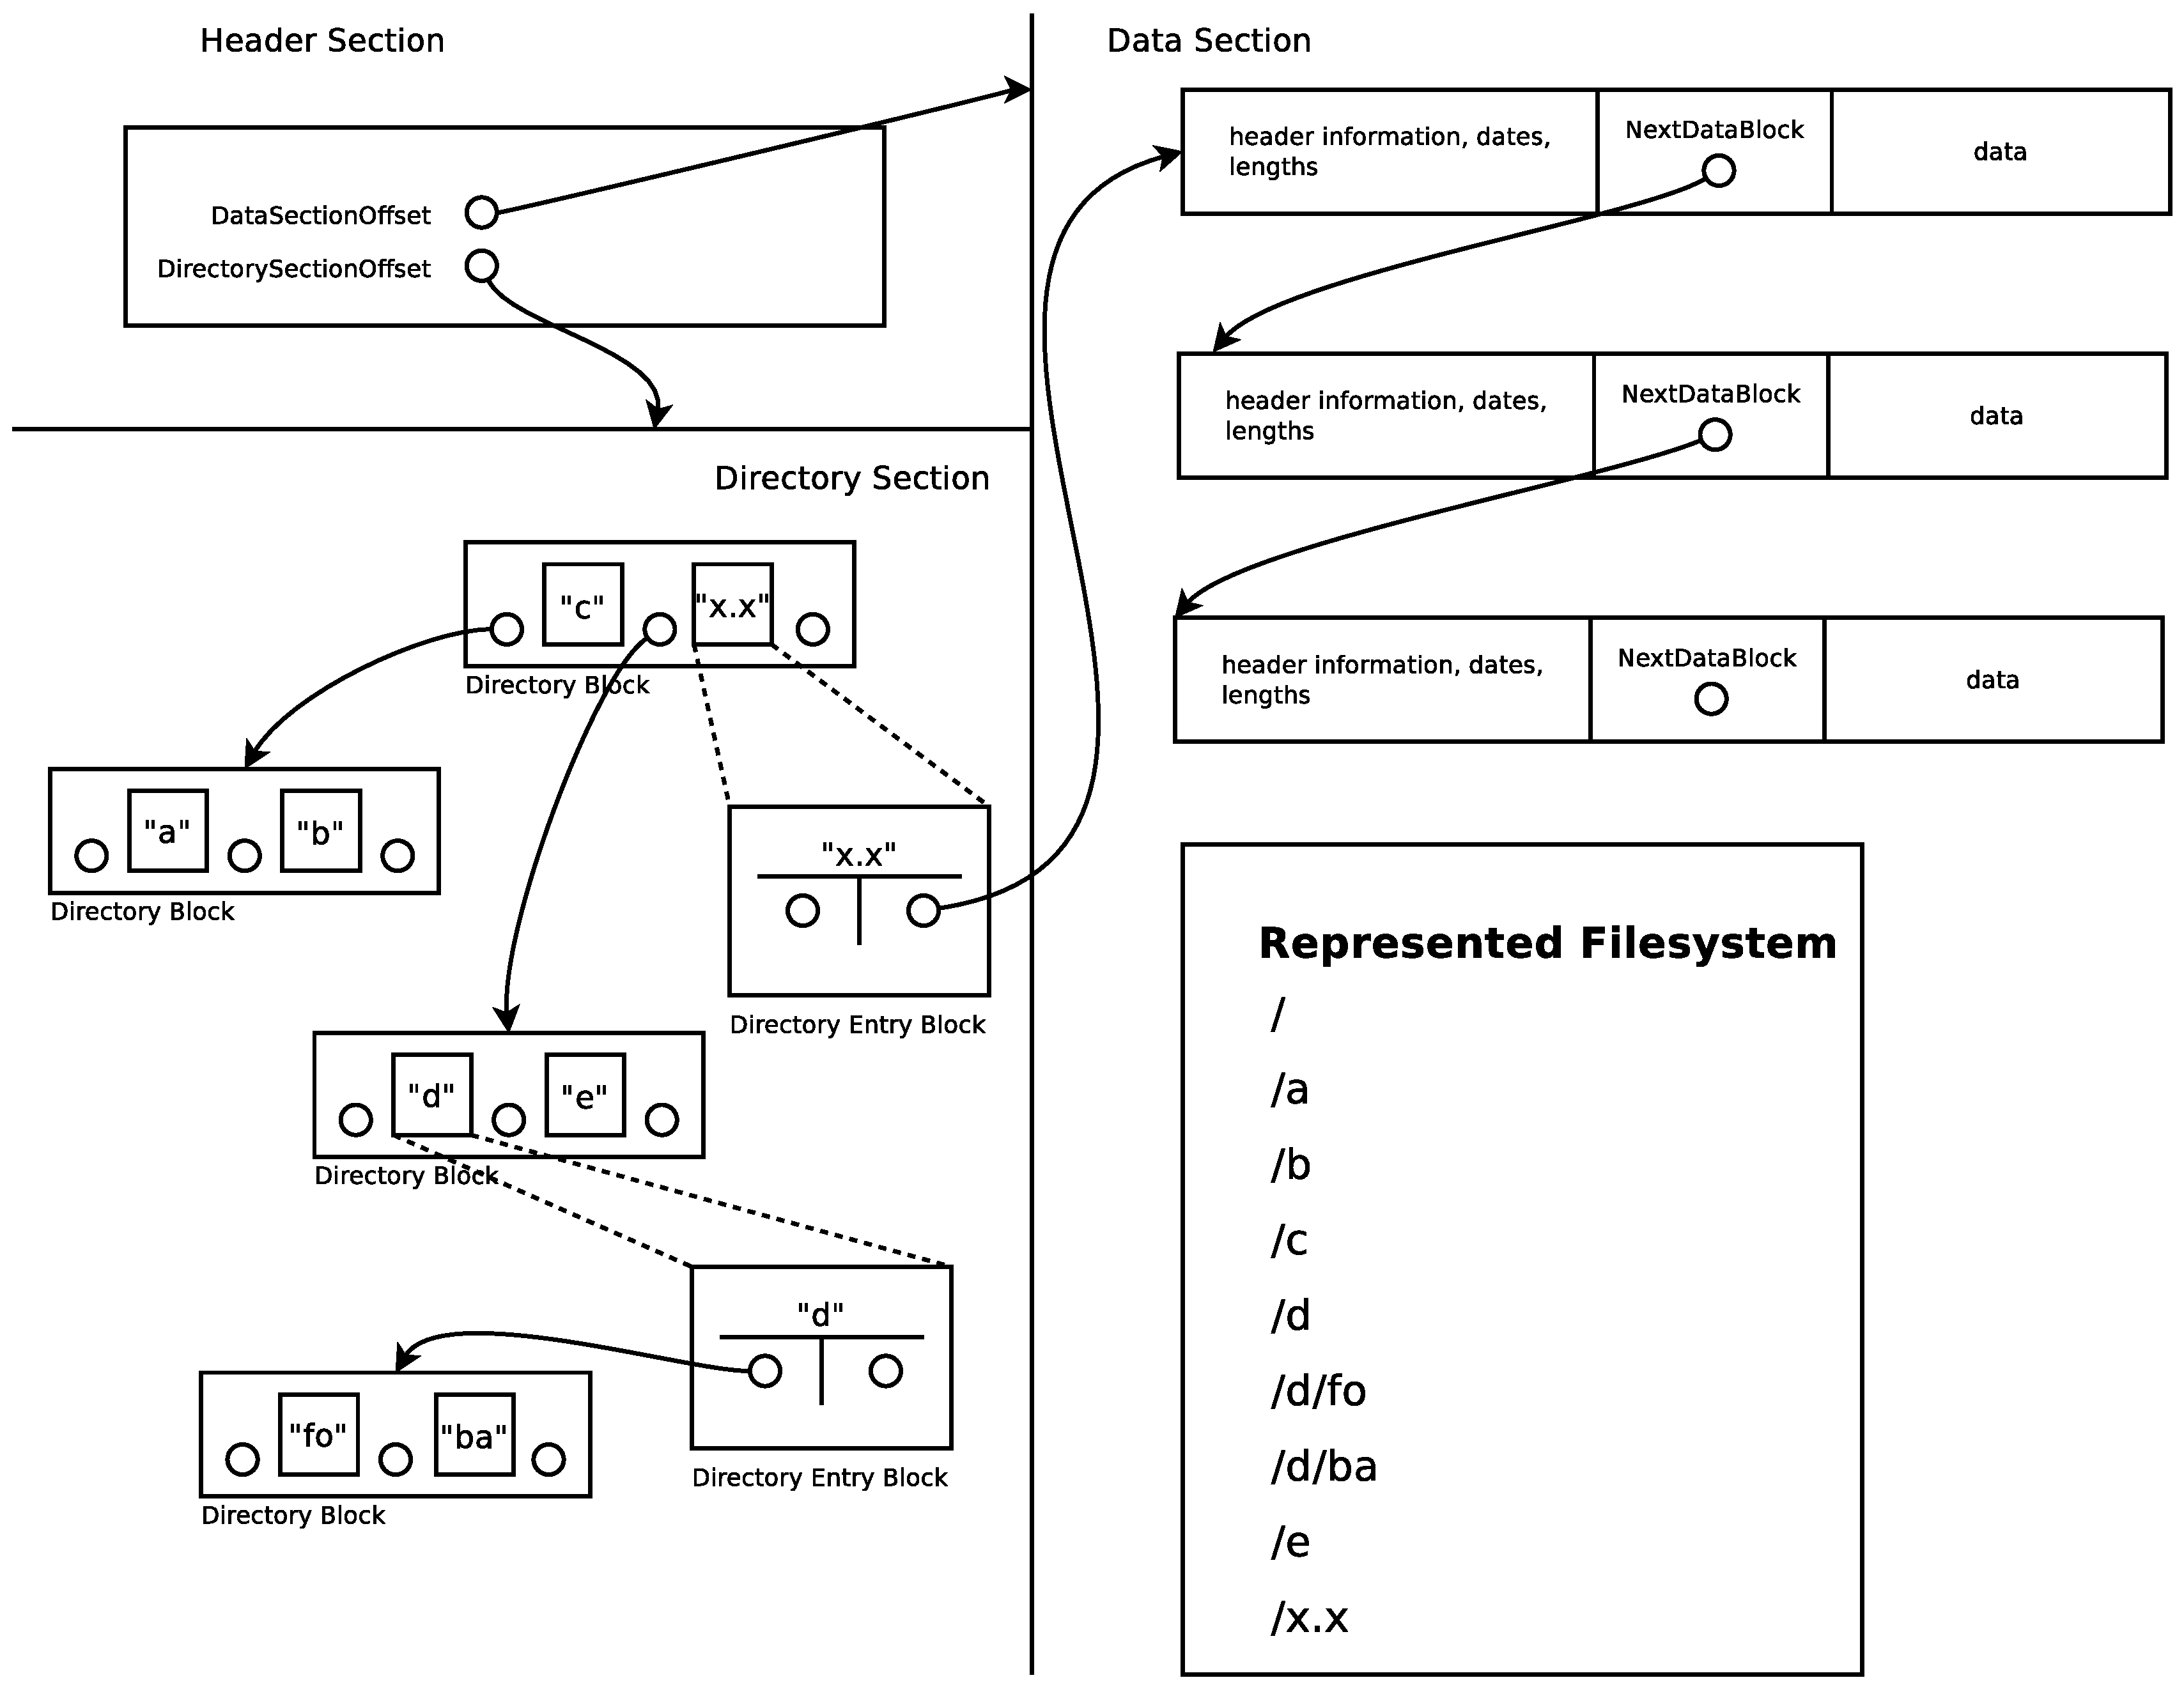
\includegraphics[width=1\textwidth]{figures/fileFormat.eps}
\caption{Overview of a disk}
\label{fig:disk_overview}
\end{figure}

\subparagraph{Header Section} The header section contains some general information
about the currently opened virtual disk. The details can be found in the
following table:

\begin{tabular}{|l|l|p{5cm}|}
\hline
\textbf{Name} & \textbf{Length} & \textbf{Description}
\\  \hline
Info & 50 byte UTF-8 String & Contains something like Badger VFS 2013 V1.0
\\ \hline
Version & 10 byte UTF-8 String & Contains something like "1.0"
\\ \hline
Compression used & 20 byte UTF-8 String & null or indicates compression used for this file
\\ \hline
Encryption used & 20 byte UTF-8 String & null or indicates encryption used for this file
\\ \hline
DirectorySectionOffset & long (8 byte) &  File offset where the directory
section starts \\ \hline
DataSectionOffset & long (8 byte) &  File offset where our data section starts
\\ \hline
 SaltString & 8 bytes  & Salt used to hash username and password randomly string generated while creating this
   file. (Not implemented yet)
 \\ \hline
  Password & xxx bytes  & CryptoHash (SHA-whatever) of Password+SaltString  (Not implemented yet)
\\ \hline

\end{tabular}


\subparagraph{Directory Section}
The directory section describes which files and folders belong to which parent
directory. This section has a fixed size and contains so called
\textit{DirectoryBlocks} which also have a fixed size. This makes management and
manipulation easy. To each directory belongs a B-Tree structure which lists all
contained entries.


\subparagraph*{DirectoryBlock}

One \textit{DirectoryBlock} represents a node in the B-Tree of order 2.

\begin{tabular}{|l|l|p{5cm}|}
\hline
\textbf{Name} & \textbf{Length} & \textbf{Description}
\\  \hline

DirectoryHeader & 1 byte & Header information. This header makes it easy to
determine whether a \textit{DirectoryBlock} is in use or not (memory
management)

\\  \hline

DirectoryEntryBlock1 & 128 byte & The smaller key inserted into the
B-Tree

\\  \hline

DirectoryEntryBlock2 & 128 byte & The bigger key inserted into the B-Tree

\\  \hline

DirectoryBlockLink1 & 8 byte & Points to another DirectoryBlock which contains
keys smaller than DirectoryEntryBlock1

\\  \hline

DirectoryBlockLink2 & 8 byte & Points to another DirectoryBlock which contains
keys bigger than DirectoryEntryBlock1 but smaller than DirectoryEntryBlock2

\\  \hline

DirectoryBlockLink3 & 8 byte & Points to another DirectoryBlock which contains
keys bigger than DirectoryEntryBlock2

\\  \hline


\end{tabular}

\subparagraph*{DirectoryEntryBlock}

Represents a single directory or file.

\begin{tabular}{|l|l|p{5cm}|}
\hline
\textbf{Name} & \textbf{Length} & \textbf{Description}
\\  \hline

Filename & 112 byte & UTF-8 file name String


\\  \hline

DataBlockLocation & 8 byte & Pointer to a DataBlock located in the Data Section.
This DataBlock holds some meta information about the current directory


\\  \hline

DirectoryEntryTreeRoot & 8 bytes & Pointer to a DirectoryBlock located in the
Directory Section. This referenced DirectoryBlock is the Root Block of a B-Tree
containing all entries of that directory specified by the current Directory Entry Block.
\newline

\textbf{This field containing a 0 indicates that this entry represents a file not a directory}



\\  \hline

\end{tabular}


\subparagraph{Data Section}
The data section is split into blocks where each of them is 1024 bytes long.
Each block contains some amount of data and points to a subsequent block (Simple
linked list).\newline\newline
Block layout \\

\begin{tabular}{|l|l|p{5cm}|}
\hline
\textbf{Name} & \textbf{Length} & \textbf{Description}
\\  \hline
BlockHeader & 1 byte &
\\
\hspace{0.2cm} 0) Header-Bit (LSB) & &  If set to 1 this is the first DataBlock
of a file.
\\
\hspace{0.2cm} 1) not used & &
\\
\hspace{0.2cm} 2) not used & &
\\
\hspace{0.2cm} 3) not used & &
\\
\hspace{0.2cm} 4) not used & &
\\
\hspace{0.2cm} 5) not used & &
\\
\hspace{0.2cm} 6) not used & &
\\
\hspace{0.2cm} 7) not used & &

\\  \hline
NextDataBlock & 8 byte &
Points to the start address of the next DataBlock (linked list).
0 if this is the last DataBlock of a certain file or folder.
\\  \hline
CreationDate & 8 byte & UTC Time when this file was created
\newline \textit{This field only exists if Header-Bit is set to 1}
\\  \hline

DataLength & 4 byte &
Indicates the number of data saved on this DataBlock.

\\  \hline
Data & n byte & user data (may be encrypted/compressed)
\\  \hline
\end{tabular}


\paragraph{The root directory}
\textbf{TODO: TEXT OR REMOVE}
